\chapter{Aufgabenstellung}
\section{Motivation}
In der medizinischen Forschung werden h�ufig Tierversuche durchgef�hrt, die am h�ufigst verwendete Tierart sind M�use und Ratten.
Die M�use und Ratten werden in K�figen gehalten, um R�ckschl�sse auf den medizinische Zustand zu erhalten wird die K�rpertemperatur gemessen. Um diesen Zeitaufwand einzusparen soll die Messung und Auswertung der Temperatur automatisiert werden. F�r diesen Zweck wurde ein Prototyp mit einer Infrarot-Kamera zur Tierbeobachtung erstellt. 
Ziel dieser Belegarbeit ist es, ein thermisches Modell zu erstellen, welches die infrarot Aufnahme einer Maus in mehreren Pixel darstellt.

\section{Beleg - Spezifikation}
Es wird f�r die erstellten Modelle eine statisch thermische Simulation durchgef�hrt. Eine Optimierung hinsichtlich der geometrischen Anordnung, sowie ein Vergleich der bisherigen Ergebnisse in Bezug auf gegenseitige Beeinflussung, zeitliche Erw�rmung und Abk�hlung. Daraufhin ist mit dem besten Ergebnis eine Simulation durchzuf�hren, die den zeitlichen Verlauf von Verschiebungseffekten sichtbar macht.
\begin{table}[bh]
	\centering
	\caption{Beleg - Spezifikation}
	\begin{tabular}{l p{9cm} } 
			\rowcolor[gray]{.8}	 Leiterplatte (LP):& 50x50 mm, 7x7 Bauelemente, 2 Lagig (Toplayer Bauelemente, Bottomlayer Leiterbahnen)\\
			Anordung& in der Mitte der LP 3x3 Pixel mit gleicher Verlustleistung (au�er das mittlere Element), �u�ere Transistorring mit maximaler Verlustleistung					\\	
			\rowcolor[gray]{.8}Ausf�hrung: & jeweils mit Transistoren SMD (SOT23) und SMD Widerst�nden (1206)\\
			Verlustleistungen:& 50 mW, 100 mW, 150 mW 
		%Feld&\multicolumn{2}{c}{}\\
	\end{tabular}
	\label{tab:beleg_anforderungen}
\end{table}

\newpage
In Abbildung \ref{fig:footprint_sot23} ist die Dimenion eines SOT23 Geh�uses und in Abbildung \ref{fig:footprint_smd1206} die Dimensionen eines SMD 1206 Widerstandes dargestellt.
\begin{center}
	\begin{minipage}[!ht]{.8\textwidth}
			\captionsetup{type=figure}
			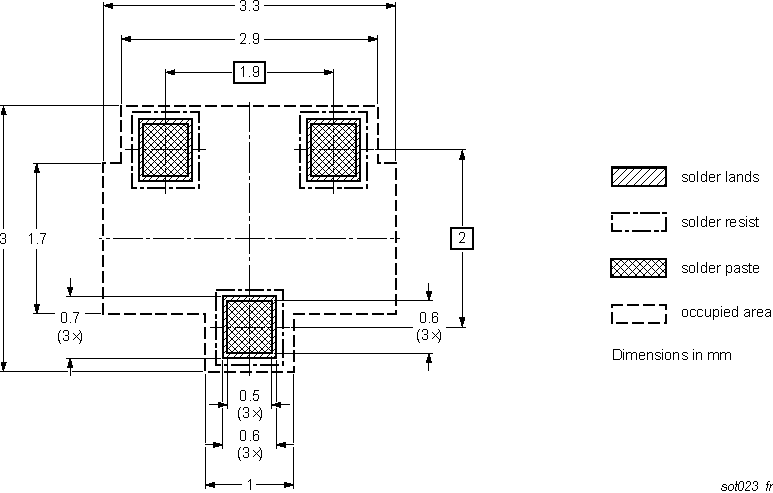
\includegraphics[width=1\linewidth]{bilder/sot23footprint.pdf}
			\caption{Transistor - Reflowfootprint SOT23 Geh�uses, Quelle: NXP - PDTC114E Datenblatt S.12}
			\label{fig:footprint_sot23}
	\end{minipage}
	\hspace{1cm}
	\begin{minipage}[!ht]{0.81\textwidth}
		\centering 
		\captionsetup{type=figure}
		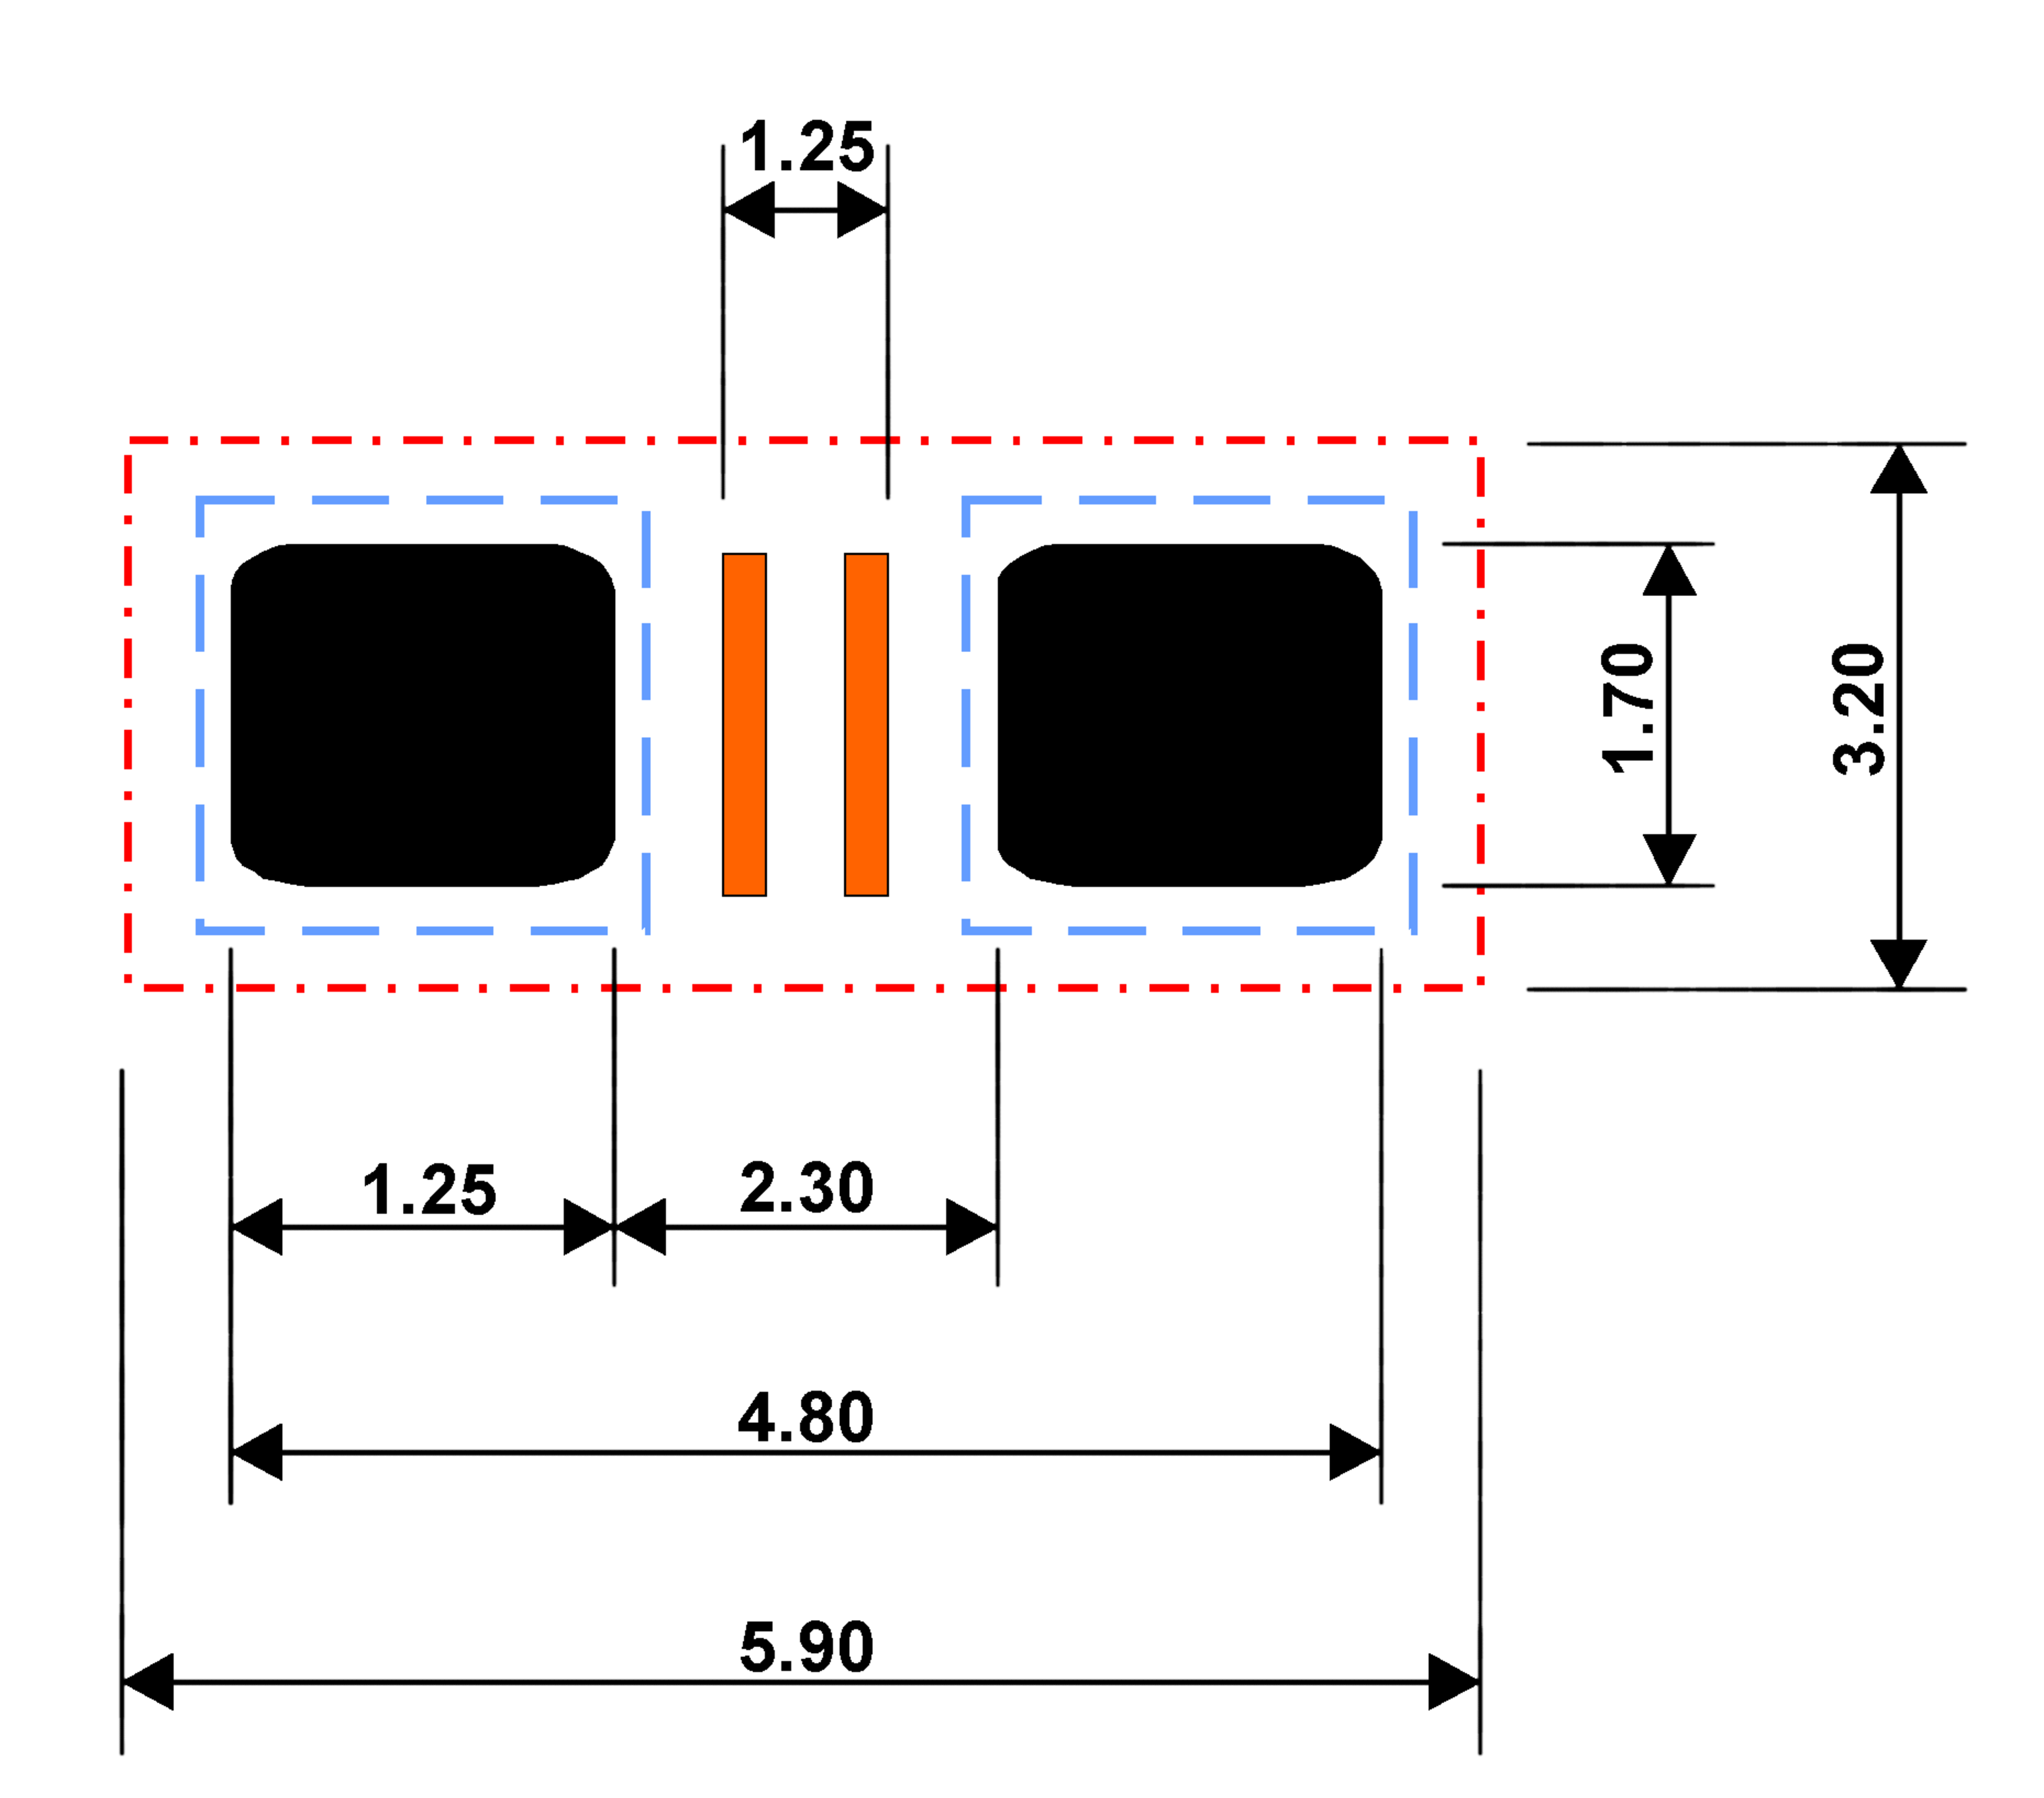
\includegraphics[width=.7\linewidth]{bilder/smd1206.pdf}
		\caption{Widerstand - Dimensionen SMD 1206, \\Quelle:\\
			\url{http://www.siongboon.com/projects/2005-09-07_home_pcb_fabrication/footprint/1206.gif}}
		%	\href{http://www.siongboon.com/projects/2005-09-07_home_pcb_fabrication/footprint/1206.gif}}
		\label{fig:footprint_smd1206}
	\end{minipage}
\end{center}


